% Paper 1 manuscript: preserving n-ary facts as hyperedges vs reifying them.
% Sources of every number: docs/hnn-ontology-encoder-v2-results.md, docs/hnn-ontology-paper1-draft-en.md (statistics),
% docs/stare-input-representation-v1-results.md, docs/stare-native-encoder-v1-results.md,
% docs/related-work-hkg-comparison.md, docs/hahe-same-harness-v1-results.md. Checked by .harness/scripts/check_paper1_manuscript_numbers.py.
% Build: .harness/scripts/build_paper1_manuscript.sh
% Revision 2 (2026-10-28): claims audited sentence by sentence against the sources (8 must-fix, 15 should-fix, 10 minor applied).
% Revision 3 (2026-11-01): HAHE run on the same pipeline and judged against our encoder (charter-hahe-same-harness-v1).
% 2026-11-04: data availability points to the public reproduction repository github.com/booobing/preserve-do-not-reify.
\documentclass[11pt,a4paper]{article}
\usepackage[T1]{fontenc}
\usepackage[utf8]{inputenc}
\usepackage{lmodern}
\usepackage[margin=25mm]{geometry}
\usepackage{amsmath,amssymb}
\usepackage{graphicx}
\usepackage{booktabs}
\usepackage{multirow}
\usepackage{threeparttable}
\usepackage[font=small,labelfont=bf]{caption}
\usepackage[authoryear,round]{natbib}
\usepackage{xcolor}
\usepackage[colorlinks=true,linkcolor=blue!50!black,citecolor=blue!50!black,urlcolor=blue!50!black]{hyperref}
\usepackage{setspace}
\usepackage{placeins}
\graphicspath{{../../outputs/hnn_ontology_figures/}}
\setstretch{1.12}
\newcommand{\hyper}{\textsf{preserve}}
\newcommand{\reif}{\textsf{reify}}
\newcommand{\prune}{\textsf{prune}}

\title{Preserve, Do Not Reify: Controlled Evidence for Keeping\\N-ary Facts Whole in Knowledge Graph Completion}
\author{[Author names]\\[2pt]\small [Affiliation, Department, City, Country]\\\small [Corresponding author e-mail]}
\date{Manuscript draft, 4 November 2026}

\begin{document}
\maketitle

\begin{abstract}
Knowledge graphs store many facts with more than two participants, and the standard way to write them down---RDF n-ary patterns, Wikidata qualifiers---\emph{reifies} each fact into an intermediate node joined to its participants by binary edges. Hyper-relational completion models instead keep the fact whole, but prior comparisons either changed the model together with the representation or, when they held the model fixed, did not use the standard reification as the control. We hold the model fixed and change only the representation. Across three studies, nine pre-registered judged comparisons and one condition pre-specified as report-only all favoured the representation that keeps the fact whole, on all five seeds. Study~1 uses one role-aware hypergraph encoder fed either hyperedges or the reified graph, under conditions that include an inductive protocol, a matched output head, a frozen sentence encoder, real Wikidata facts and a reified control with twice the depth. Study~2 leaves the public StarE code unmodified, runs its standard protocol on WD50K(100) and swaps only the graph its encoder sees; the native graph reaches test MRR 0.6553, reproducing the published 0.654, against 0.6485 for the reified graph. Study~3 places our encoder inside the same pipeline: preserving reaches 0.6648, reifying 0.6561 and removing qualifiers from the encoder 0.6519. At the standard budget the gaps are small (0.007--0.013 MRR) but never reverse. With StarE's encoder, however, the reified graph learns faster---a 76-epoch pilot had it ahead by 0.098 MRR---so short-budget comparisons can report the opposite order. We claim neither state-of-the-art accuracy---HAHE's public code, run on the identical pipeline, beats our encoder on all five seeds (0.6784 vs.\ 0.6648)---nor any retrieval benefit; under a frozen sentence encoder, a structure-free text baseline retrieves facts better than every structured variant.
\end{abstract}

\noindent\textbf{Keywords:} N-ary knowledge graph completion; hyper-relational knowledge graph; reification; hypergraph neural network; link prediction; controlled comparison

\section{Introduction}

Many facts in a knowledge base have more than two participants. ``Kim led the research lab as team lead from 2021 to 2023'' is one fact about a person, an organisation, a role and a time span, not four separate facts. The data models that store such facts offer binary edges: an RDF property is a binary relation \citep{cyganiak2014rdf}, a W3C Working Group Note describes writing n-ary relations through an intermediate individual \citep{noy2006nary}, and Wikidata attaches qualifiers to a main statement \citep{vrandecic2014wikidata}. In each case one fact is \emph{reified}: a node stands for the fact and binary edges connect it to each participant. This practice reflects the binary data model, not evidence about what a learned model needs.

Link prediction on n-ary facts has moved the other way. Embedding models score whole n-ary tuples \citep{wen2016mtransh,guan2019nalp,fatemi2020hype}, convolutional and attention models read a main triple together with its qualifiers \citep{rosso2020hinge,wang2021gran,hu2023hyperformer}, and message-passing models propagate information across facts while keeping qualifiers attached \citep{galkin2020stare,luo2023hahe,lee2025maypl,lee2026krepe,ji2026glore}. These models rest on the premise that keeping a fact whole is better than splitting it. The direct evidence for the premise is thinner than the volume of work suggests. When HINGE was compared with reified inputs, the reified inputs went to different (binary) models \citep{rosso2020hinge}; when m-TransH compared decompositions, adding a fact node to the n-ary data \emph{improved} accuracy \citep{wen2016mtransh}; and a recent analysis found that a qualifier-free path-based GNN matches or exceeds specialised hyper-relational models on WD50K \citep{wang2025understanding}. None of these holds the model fixed and swaps a preserved fact for its standard reification.

We do exactly that. Our question is narrow: \emph{with the encoder, its training budget and the information it receives held fixed, and its parameter count fixed or within a few percent, does it matter whether an n-ary fact enters whole or as its standard reification?} We answer it three times, with increasingly standard machinery.

\begin{itemize}
\item \textbf{Study 1} uses one role-aware hypergraph encoder and changes only its input graph. Six conditions were judged---the baseline, an inductive protocol, a matched output head, a frozen multilingual sentence encoder, real Wikidata facts (WD50K(100)), and a reified control with twice the layers and 14\% more parameters---and a seventh, the three synthetic controls combined, was pre-specified as report-only.
\item \textbf{Study 2} leaves the public StarE code \citep{galkin2020stare} unmodified, runs its standard protocol and budget, and swaps the encoder graph for the reified one through a one-method subclass that runs StarE's own qualifier-free convolution on it.
\item \textbf{Study 3} places the encoder of Study~1 inside the same standard pipeline and adds a third arm that removes the qualifiers from the encoder graph, addressing the qualifier-free result of \citet{wang2025understanding}.
\end{itemize}

To place the encoder among published models, we also run HAHE's public code \citep{luo2023hahe} on the identical pipeline and judge it against our encoder by the same rule. That comparison is between models, not representations, and it is not one of the nine.

Our contributions are as follows.
\begin{enumerate}
\item A controlled comparison in which the representation is the only intended difference. Nine two-arm comparisons were judged by a rule fixed before the runs, and all nine---together with the report-only combined condition---favoured the unreified representation (a hyperedge in Studies~1 and~3, StarE's qualifier-carrying edge in Study~2) on 5 of 5 seeds.
\item Replication outside our own code and protocol. The direction holds on an external backbone whose published number we reproduce (0.6553 vs.\ 0.654), and for our encoder under the same standard protocol.
\item A budget effect that can flip conclusions. With StarE's encoder the reified graph learns faster early in training: a 76-epoch pilot had it ahead by 0.098 MRR, and in the full runs it leads at most evaluation points before epoch 120. Comparisons run on short budgets can therefore report the opposite of the converged order.
\item An honest position in the literature. On WD50K(100) our encoder sits at the level of StarE, below HAHE when we run HAHE's public code on the identical pipeline (5 of 5 seeds), and far below GLoRE; we report where a structure-free text encoder beats every structured variant, and where an attempt to carry the advantage into a language model failed.
\end{enumerate}

\section{Related work}

\paragraph{N-ary and hyper-relational completion.}
Three formalisms coexist. Role--value formulations treat a fact as a set of role:value pairs \citep{guan2019nalp,guan2021relatedness}; knowledge hypergraphs treat it as a relation over an ordered tuple \citep{wen2016mtransh,fatemi2020hype}; hyper-relational graphs keep a main triple and attach qualifier pairs \citep{rosso2020hinge,galkin2020stare}. Within the last family, models differ in how a qualifier enters. StarE folds qualifier pairs into the feature of the main edge of a CompGCN-style encoder \citep{vashishth2020compgcn,galkin2020stare}, so a qualifier value contributes to messages but receives none from its own statement. GRAN treats each fact as a small heterogeneous graph processed by edge-biased attention \citep{wang2021gran}, and HyperFormer combines a token sequence with one-hop neighbour aggregation \citep{hu2023hyperformer}. HAHE adds a global hypergraph in which qualifier values are members of the fact \citep{luo2023hahe}; MAYPL passes messages over structure induced by qualifiers \citep{lee2025maypl}; KREPE sums relation--entity pairs into a fact representation and passes context messages across facts \citep{lee2026krepe}; and GLoRE encodes relation--entity pairs jointly at a global and a local level \citep{ji2026glore}. HEHRGNN treats each fact as a hyperedge hub \citep{rajagopalamenon2026hehrgnn}, and hyper-relational structure has been used in applications such as next-POI recommendation \citep{zhang2023hkgnn}. The encoder we study belongs to the participant family: every participant of a fact sends and receives messages through the fact.

\paragraph{Evidence about the representation itself.}
\citet{wen2016mtransh} compared the same model family on JF17K converted three ways: a pairwise (star-to-clique) expansion reached Hits@10 49.26\%, direct n-ary instances 68.73\%, and n-ary instances with an added fact-ID role 80.82\%. The last result points in the direction opposite to ours, but the fact node there is \emph{added} to an intact n-ary fact, whereas reification \emph{replaces} the fact by the node and its binary edges. \citet{rosso2020hinge} gave eight binary embedding models a reified version of each fact; reification did not help them, and HINGE, a different model, beat all of them. \citet{fatemi2020hype} showed that existing embedding methods do not work well out of the box on graphs binarised by reification. \citet{galkin2020stare} showed that removing qualifiers from StarE costs a large margin on WD50K(100) (0.654 vs.\ 0.380 MRR), and \citet{wang2025understanding} found that NBFNet \citep{zhu2021nbfnet} without qualifiers (0.360 on WD50K) matches or exceeds StarE as re-run by those authors (0.346; originally 0.349), and that adding qualifiers as extra triples makes NBFNet worse. The GLoRE authors report that node-centric global aggregation confuses roles and loses 0.13 MRR on WD50K against pair-based aggregation (0.348 vs.\ 0.478) \citep{ji2026glore}. Each of these varies something besides the representation, or varies the representation without the standard reification as the control.

\paragraph{Hypergraph neural networks.}
Our encoder lies in the design space of HGNN, UniGNN, AllSet and multi-relational hypergraph message passing \citep{feng2019hgnn,huang2021unignn,chien2022allset,yadati2020gmpnn}; see \citet{kim2024hgnnsurvey} for a taxonomy. We do not propose a new architecture; the comparison only requires that both arms use the same one.

\section{Representations and encoder}

\subsection{Three views of the same fact}

A fact $f$ has a relation $r_f$ and members $\{(v_1,\rho_1),\dots,(v_k,\rho_k)\}$, where $\rho_i$ is the role of entity $v_i$ (subject, object, or a qualifier property). Figure~\ref{fig:repr} shows the two views compared throughout.

\begin{itemize}
\item \textbf{\hyper} (hyperedge). $f$ is one hyperedge of type $r_f$ whose incidences carry the roles $\rho_i$. All members meet in one message-passing hop.
\item \textbf{\reif} (standard reification). $f$ becomes a statement node $b_f$, and each member becomes a binary edge $(b_f, v_i)$ whose \emph{type} encodes $\rho_i$; the incidences of these edges carry only the generic roles subject and object. The statement node carries $r_f$, as the type triple of classic reification does. No information is lost, since $f$ can be read back from $b_f$ and its edges, but members are now two hops apart.
\item \textbf{\prune} (Study~3 only). $f$ is a hyperedge over its subject and object; qualifiers are absent from the encoder graph. In Study~3 the decoder still receives the qualifier tokens, so this arm isolates what qualifier \emph{structure in the encoder} adds.
\end{itemize}

\begin{figure}[t]
\centering
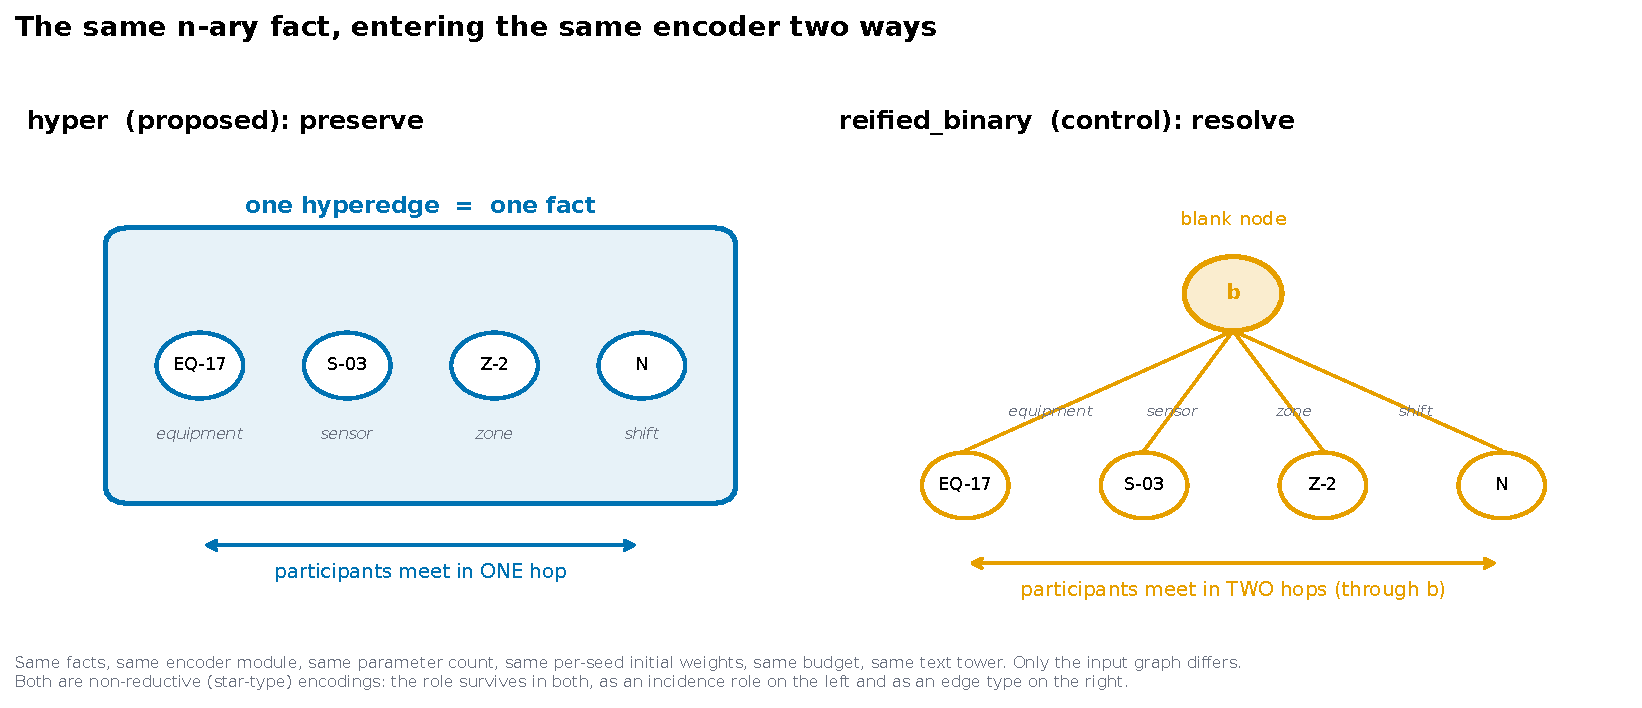
\includegraphics[width=0.86\linewidth]{paper1_fig1_representation.pdf}
\caption{The same n-ary fact entering the same encoder in two ways. Left (\hyper): one hyperedge, members meet in one hop. Right (\reif): a statement node with one binary edge per member, members two hops apart. Roles survive on both sides---as incidence roles on the left, as edge types on the right. What differs is the path, not the information.}
\label{fig:repr}
\end{figure}

\subsection{Role-aware hypergraph encoder}

The encoder of Studies~1 and~3 alternates node-to-edge and edge-to-node updates. With $E_{\text{role}}$ a role embedding and $\phi_{1..4}$ linear maps, each layer computes
\begin{align}
m_e &= \operatorname{mean}_{v \in e}\, \sigma\!\left(\phi_1(h_v + E_{\text{role}}[\rho_{v,e}])\right), \qquad h_e \leftarrow \operatorname{LN}\!\left(h_e + \phi_2([h_e; m_e])\right),\\
m_v &= \operatorname{mean}_{e \ni v}\, \sigma\!\left(\phi_3(h_e + E_{\text{role}}[\rho_{v,e}])\right), \qquad h_v \leftarrow \operatorname{LN}\!\left(h_v + \phi_4([h_v; m_v])\right),
\end{align}
with GELU $\sigma$ and layer normalisation LN; the edge-to-node step uses the updated $h_e$, and two layers are stacked. Edges start from a relation embedding, $h_e^{0} = E_{\text{rel}}[r_e]$, and node states pass through an input layer normalisation. The same module consumes either view; only the incidence list differs. In the reified view the statement node is an ordinary node and its binary edges are ordinary two-member hyperedges.

In Study~1, nodes start from a type embedding plus a projected text embedding, and completion scores candidate nodes against a query built from the fact's hidden state and the masked role. The fact embedding is aligned with sentence embeddings of the fact by CLIP-style contrastive learning \citep{radford2021clip}, which defines the retrieval task. \hyper\ reads the fact through the edge head $W_e h_e$. In the baseline and in conditions A and C the reified arm reads $h_{b_f}$ through the node head; condition B, and with it D, the combined condition and the depth condition, applies the same edge head to $h_{b_f}$. The default text tower is a hashed n-gram encoder; condition C replaces it with the frozen sentence encoder paraphrase-multilingual-MiniLM-L12-v2 \citep{reimers2019sbert}. A structure-free reference line (\textsf{flat\_text}) encodes only the fact sentence through an MLP of matching size; it is reported but never judged.

In Study~3 the encoder replaces StarE's convolution: nodes start from StarE's learned entity table, a statement node starts from its relation's edge embedding plus one shared learned vector, StarE's dropout is applied after each layer, and StarE's Transformer decoder reads the output node table unchanged.

\subsection{Fairness conditions}

In Study~1 both arms share the module, the vocabulary, the parameter count (351,553), the per-seed initial weights, the budget and the text encoder; automated tests pin these conditions. In Study~3 the three arms share every module and differ in parameter count only by the 200-dimensional shared vector of \reif\ (5,318,216 vs.\ 5,318,416). In Study~2 the native StarE encoder has 1.6\% more parameters than the reified arm, because the reified graph needs no qualifier aggregation weights (5,068,016 vs.\ 4,989,016).

\section{Experimental design}

\subsection{Data}

The synthetic world has 78 entities and 390 n-ary facts with template sentences (272 training, 59 validation and 59 test facts), which define both a retrieval task (find a fact from a sentence) and a completion task. WD50K(100) is the subset of the StarE release in which every statement has at least one qualifier \citep{galkin2020stare}: 31,314 statements (22,738/3,279/5,297), 18,791 entities across all positions, of which 7,917 appear only as qualifier values, 204 predicates and 134 qualifier properties. Study~1's loader keeps the first value of a repeated qualifier property within a statement, giving 18,025 entities and mean arity 3.30; Studies~2 and~3 use StarE's own loader, which keeps repeats and caps a statement at six qualifier pairs.

\subsection{Three studies}

Table~\ref{tab:design} summarises the design. Studies~2 and~3 follow StarE's standard protocol exactly: the subject or object of each test statement is masked (both directions are evaluated), candidates are all entities except those that appear only as qualifier values, ranking is filtered \citep{bordes2013transe}, the graph contains train and validation statements, and training runs StarE's default budget (401 epochs, batch 128, Adam with learning rate $10^{-4}$, label smoothing 0.1). Study~1 uses its own protocol, described in Section~\ref{sec:position}.

\begin{table}[t]
\centering
\footnotesize
\caption{Design of the three studies. All judged comparisons use seeds 1--5.}
\label{tab:design}
\begin{tabular}{@{}p{1.9cm}p{4.2cm}p{4.2cm}p{4.2cm}@{}}
\toprule
 & Study 1 & Study 2 & Study 3 \\
\midrule
Encoder & role-aware hypergraph encoder ($d=64$, 2 layers) & StarE, unmodified files ($d=200$) & role-aware hypergraph encoder ($d=200$, 2 layers) \\
Decoder & completion query $\cdot$ node embeddings & StarE Transformer & StarE Transformer \\
Arms & \hyper\ vs.\ \reif & native graph vs.\ \reif & \hyper\ vs.\ \reif; \hyper\ vs.\ \prune \\
Data & synthetic world; WD50K(100) & WD50K(100) & WD50K(100) \\
Protocol & own (any role masked, all entities, filtered; WD50K: 2,000 sampled test facts) & StarE standard (subject/object, filtered, full test set) & StarE standard \\
Budget & 1,500 steps, batch 32 & 401 epochs & 401 epochs \\
Judged metrics & recall@5 and acc@1 (synthetic); MRR and Hits@10 (WD50K) & test MRR and Hits@10 at epoch 401 & test MRR and Hits@10 at epoch 401 \\
\bottomrule
\end{tabular}
\end{table}

\subsection{Positioning run: HAHE on the same pipeline}
\label{sec:hahe-design}

The published WD50K(100) values of the strongest models exist only as a figure, and a gap of a few thousandths of MRR could come from protocol differences alone. We therefore ran HAHE \citep{luo2023hahe}, which combines hypergraph attention over a global graph of training facts (by its default, the first fifth of them) with a 12-layer Transformer over each fact, on the pipeline of Studies~2 and~3. Its five source files are imported unmodified at a pinned commit (\texttt{e35e0a7b}) and fed the rows produced by StarE's loader, so the training graph, the 10,594 test queries, the 10,874 candidate entities and the filter are those of Studies~2 and~3; each StarE entity maps to one HAHE token, and automated tests check the mapping. HAHE scores its whole vocabulary; we take the entity scores and rank them with StarE's rule, which our tests check against StarE's formula on random scores.

Training follows HAHE's published WD50K recipe without tuning (hidden size 256, AdamW with a one-cycle schedule, batch 512, 300 epochs; no WD50K(100) recipe exists). HAHE's objective masks every position of a fact---subject, relation, object, qualifier properties and values---which gives 298 optimiser steps per epoch, and the model has 26,584,063 parameters, five times the 5,318,216 of our encoder. We compare HAHE at epoch 300 with \hyper\ of Study~3 at epoch 401. Epochs are not matched, because the two models train on different queries and an epoch is not the same amount of training; we report steps, compute and the learning curve instead. As a check on the port, we also score HAHE with its own ranking rule (all 18,791 entities as candidates, ties counted against the target) and compare it with the GLoRE authors' re-run \citep{ji2026glore}; agreement within $\pm$0.03 was fixed in advance as the criterion, reported but not judged.

\subsection{Judging rule and pre-registration}
\label{sec:judging}

A seed is won by the arm that is strictly better on it; ties count for nobody. An arm wins a comparison only if it wins \emph{both} judged metrics on at least 4 of 5 seeds; otherwise the result is ``no consistent order''. In Study~1 the rule was one-sided (does \hyper\ beat \reif?). In Studies~2 and~3 and in the HAHE comparison it was two-sided; our predictions, recorded before the runs, favoured \reif\ in Study~2 (55\%), \hyper\ in Study~3 (60\%) and HAHE over our encoder (50\%, against 30\% for no consistent order). Arms, metrics, budgets and seeds were never changed after results were seen.

The plans were written in versioned documents (``charters''). How far an outsider can verify their timing differs by study, and none of them sits on a third-party registry. Study~1's baseline plan was committed together with its result, and the v2 charter covering conditions A--D and the combined condition was committed before those conditions were implemented (commit \texttt{c054b59d5}, 20 August 2026; results 22 August), after the baseline's direction was known. The depth condition's charter is dated before its run but was first committed together with its results. For Study~2, the judged-run rule entered the repository's event log before the first judged run finished and was committed with the results; for Study~3 and for the HAHE comparison of Section~\ref{sec:position}, the charter and event-log entries precede the runs and are committed with the results. The statistical tests of Section~\ref{sec:study1} were planned after the Study~1 verdicts but committed before any test statistic was computed (commit \texttt{24b2e1f71}).

Beyond the rule we report seed-paired differences with 95\% confidence intervals and two-sided $t$-tests (4 degrees of freedom), and an exact sign-flip test. Table~\ref{tab:stats} reports $\hyper - \text{control}$, so positive values favour \hyper; Table~\ref{tab:std} reports $\text{control} - \hyper$, so negative values favour \hyper. With five seeds the smallest attainable sign-flip $p$ is $2/32 = 0.0625$, so that test confirms only that all seeds agree in direction. Reporting seed variation follows \citet{bouthillier2021variance}.

\subsection{Implementation}

All runs used one 8~GB RTX~3060~Ti. Study~1 ran in PyTorch's deterministic mode. Studies~2 and~3 use StarE at commit \texttt{b294b9e2} with PyTorch~2.10 and PyTorch Geometric~2.6.1; the three \texttt{torch\_scatter} functions StarE uses are replaced by native PyTorch equivalents, checked against explicit loops. To avoid hardware resets under sustained load, the runs idle the GPU for 150~ms after each optimiser step and checkpoint every five epochs; the idle time does not change the computation. One Study~3 run (\reif, seed~1) was resumed from its epoch-30 checkpoint after a machine reset. The HAHE runs use the same schedule and also checkpoint the optimiser, learning-rate schedule, random-number and data-shuffling states; two of them were resumed, one after an application restart and one after a machine reset, and in both the training loss of the first resumed epoch matched the value recorded before the interruption.

\section{Results}

\subsection{Study 1: one encoder, seven conditions}
\label{sec:study1}

Table~\ref{tab:study1} lists the seven conditions. A, B and C each change one thing relative to the baseline. D uses real data under the inductive protocol with the matched head. The depth condition changes only depth relative to B, and the report-only combined condition applies A, B and C together. \hyper\ won both metrics on 5 of 5 seeds in every condition (Figure~\ref{fig:gap}).

\begin{table}[t]
\centering
\caption{Study 1. Means over five seeds; the control is \reif\ in every row (its four-layer variant in the last row). In every condition \hyper\ wins both metrics on 5/5 seeds.}
\label{tab:study1}
\footnotesize
\begin{tabular}{@{}lp{4.4cm}lcc@{}}
\toprule
Condition & What is controlled & Metrics & \hyper & control \\
\midrule
Baseline & --- & recall@5 / acc@1 & \textbf{0.863 / 0.502} & 0.670 / 0.424 \\
A: inductive & evaluated facts' structure removed from training & recall@5 / acc@1 & \textbf{0.870 / 0.310} & 0.723 / 0.212 \\
B: head parity & control reads through the same output head & recall@5 / acc@1 & \textbf{0.863 / 0.502} & 0.699 / 0.403 \\
C: frozen text & frozen multilingual sentence encoder & recall@5 / acc@1 & \textbf{0.846 / 0.405} & 0.585 / 0.251 \\
D: real data & WD50K(100), inductive, matched head & MRR / Hits@10 & \textbf{0.147 / 0.289} & 0.118 / 0.215 \\
A+B+C (reported) & three synthetic controls together; pre-specified as report-only & recall@5 / acc@1 & \textbf{0.815 / 0.234} & 0.605 / 0.178 \\
Depth + parity & control has 4 layers, +14\% parameters, matched head & recall@5 / acc@1 & \textbf{0.863 / 0.502} & 0.672 / 0.400 \\
\bottomrule
\end{tabular}
\end{table}

\begin{figure}[t]
\centering
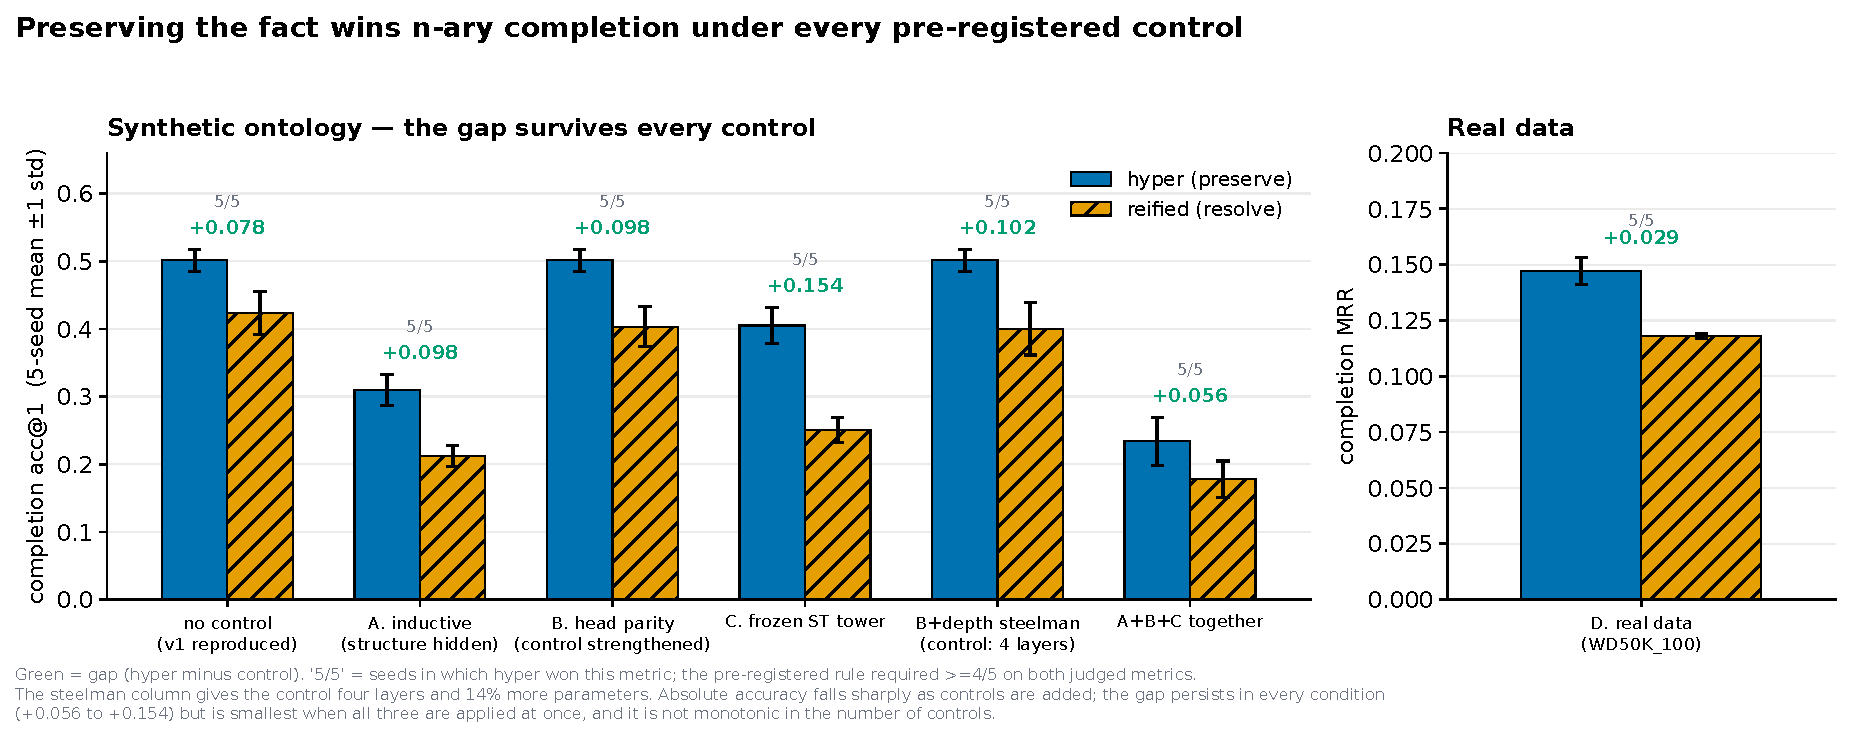
\includegraphics[width=0.92\linewidth]{paper1_fig2_gap_across_controls.pdf}
\caption{Study 1: completion per condition (mean over five seeds, $\pm$1 s.d.). Absolute accuracy falls as controls are added, but a gap remains in every condition (+0.056 to +0.154). The right panel is WD50K(100) with MRR, on its own axis.}
\label{fig:gap}
\end{figure}

Three readings follow. First, the controls make the task harder: completion accuracy falls from 0.502 to 0.310 under the inductive protocol and to 0.234 with three controls. Second, the gap does not shrink with it; under the inductive protocol it grows from +0.078 to +0.098. Third, two alternative explanations fail in this synthetic setting. Matching the control's output head raised its retrieval slightly and lowered its completion, leaving the gap in place. Giving the control twice the layers and 14\% more parameters, together with the matched head, \emph{widened} the completion gap from +0.098 to +0.102; the charter had fixed, before the run, that a reduction below 25\% would mean depth does not explain the gap. Depth alone (without head parity) narrowed it by only 9\% (+0.078 to +0.071).

Table~\ref{tab:stats} gives the seed-paired tests. All 14 pairs remain significant after Holm correction \citep{holm1979}, and all have sign-flip $p = 0.0625$. Two are borderline: completion under A+B+C (confidence interval lower bound +0.003) and retrieval under C (Holm $p = 0.043$, wide interval). In the hardest condition the direction is consistent but the size cannot be distinguished from values near zero, and we rest no claim on it.

\begin{table}[t]
\centering
\small
\caption{Study 1: seed-paired tests (difference = \hyper\ $-$ control; two-sided $t$, 4 d.f.; Holm correction across the 14 pairs).}
\label{tab:stats}
\begin{tabular}{@{}llcccc@{}}
\toprule
Condition & Metric & Mean difference [95\% CI] & $t(4)$ & $p$ (Holm) & $d_z$ \\
\midrule
Baseline & recall@5 & +0.193 [+0.121, +0.265] & 7.43 & 0.016 & 3.32 \\
Baseline & acc@1 & +0.078 [+0.046, +0.110] & 6.78 & 0.020 & 3.03 \\
A: inductive & recall@5 & +0.147 [+0.100, +0.194] & 8.67 & 0.010 & 3.88 \\
A: inductive & acc@1 & +0.098 [+0.058, +0.139] & 6.74 & 0.020 & 3.02 \\
B: head parity & recall@5 & +0.164 [+0.095, +0.233] & 6.57 & 0.020 & 2.94 \\
B: head parity & acc@1 & +0.098 [+0.079, +0.117] & 14.28 & 0.002 & 6.39 \\
C: frozen text & recall@5 & +0.262 [+0.064, +0.459] & 3.67 & 0.043 & 1.64 \\
C: frozen text & acc@1 & +0.154 [+0.127, +0.181] & 15.72 & 0.001 & 7.03 \\
D: real data & MRR & +0.029 [+0.022, +0.036] & 11.97 & 0.003 & 5.35 \\
D: real data & Hits@10 & +0.074 [+0.065, +0.083] & 22.26 & $<$0.001 & 9.96 \\
A+B+C & recall@5 & +0.210 [+0.089, +0.332] & 4.80 & 0.033 & 2.15 \\
A+B+C & acc@1 & +0.056 [+0.003, +0.109] & 2.93 & 0.043 & 1.31 \\
Depth + parity & recall@5 & +0.191 [+0.101, +0.282] & 5.89 & 0.021 & 2.63 \\
Depth + parity & acc@1 & +0.102 [+0.044, +0.160] & 4.86 & 0.033 & 2.17 \\
\bottomrule
\end{tabular}
\end{table}

\subsection{Study 2: an external encoder with unmodified code}

Table~\ref{tab:std} (upper block) gives the result. StarE's native graph beat the reified graph on both metrics on 5 of 5 seeds: test MRR 0.6553 vs.\ 0.6485, paired difference $-0.0068$ (95\% CI $-0.0104$ to $-0.0031$, $p = 0.0067$), and Hits@10 0.7766 vs.\ 0.7708 ($-0.0058$, CI $-0.0073$ to $-0.0043$). The native arm reproduces the published 0.654 \citep{galkin2020stare} to within 0.002, so the port is faithful.

The learning curves (Figure~\ref{fig:curves}a) show why the budget matters. Averaged over seeds, the reified graph leads at epochs 10--20 and again from epoch 60 to epoch 110, by about 0.09 MRR at 70--80 epochs; the native graph leads briefly at 30--50 epochs and then from epoch 120 to the end. A pilot planned before the judged runs (one seed, 76 epochs, training graph only, validation set) had recorded the reified graph ahead at 0.434 vs.\ 0.336---the opposite of the converged verdict. We report both because both are true at their budgets.

\begin{table}[t]
\centering
\small
\caption{Studies 2 and 3: WD50K(100), StarE standard protocol, test set, epoch 401, mean $\pm$ s.d.\ over seeds 1--5. Paired difference = control $-$ \hyper\ (or native StarE graph); negative values favour \hyper. Per-seed values are in Appendix~\ref{app:seeds}.}
\label{tab:std}
\begin{tabular}{@{}llcccc@{}}
\toprule
& Arm & MRR & Hits@1 & Hits@10 & Seeds won \\
\midrule
\multirow{2}{*}{Study 2 (StarE)} & native graph & \textbf{0.6553 $\pm$ 0.0013} & \textbf{0.5891} & \textbf{0.7766} & 5/5, 5/5 \\
& \reif & 0.6485 $\pm$ 0.0021 & 0.5809 & 0.7708 & --- \\
\midrule
\multirow{3}{*}{Study 3 (ours)} & \hyper & \textbf{0.6648 $\pm$ 0.0026} & \textbf{0.6025} & \textbf{0.7777} & 5/5, 5/5 (both) \\
& \reif & 0.6561 $\pm$ 0.0024 & 0.5942 & 0.7686 & --- \\
& \prune & 0.6519 $\pm$ 0.0026 & 0.5871 & 0.7709 & --- \\
\midrule
\multicolumn{6}{@{}l}{\emph{Paired differences (MRR; Hits@10), 95\% CI}} \\
\multicolumn{2}{@{}l}{Study 2: \reif\ $-$ native} & \multicolumn{4}{l}{$-0.0068$ [$-0.0104$, $-0.0031$]; \ $-0.0058$ [$-0.0073$, $-0.0043$]} \\
\multicolumn{2}{@{}l}{Study 3: \reif\ $-$ \hyper} & \multicolumn{4}{l}{$-0.0087$ [$-0.0110$, $-0.0065$]; \ $-0.0092$ [$-0.0106$, $-0.0077$]} \\
\multicolumn{2}{@{}l}{Study 3: \prune\ $-$ \hyper} & \multicolumn{4}{l}{$-0.0129$ [$-0.0171$, $-0.0087$]; \ $-0.0069$ [$-0.0107$, $-0.0031$]} \\
\bottomrule
\end{tabular}
\end{table}

\begin{figure}[t]
\centering
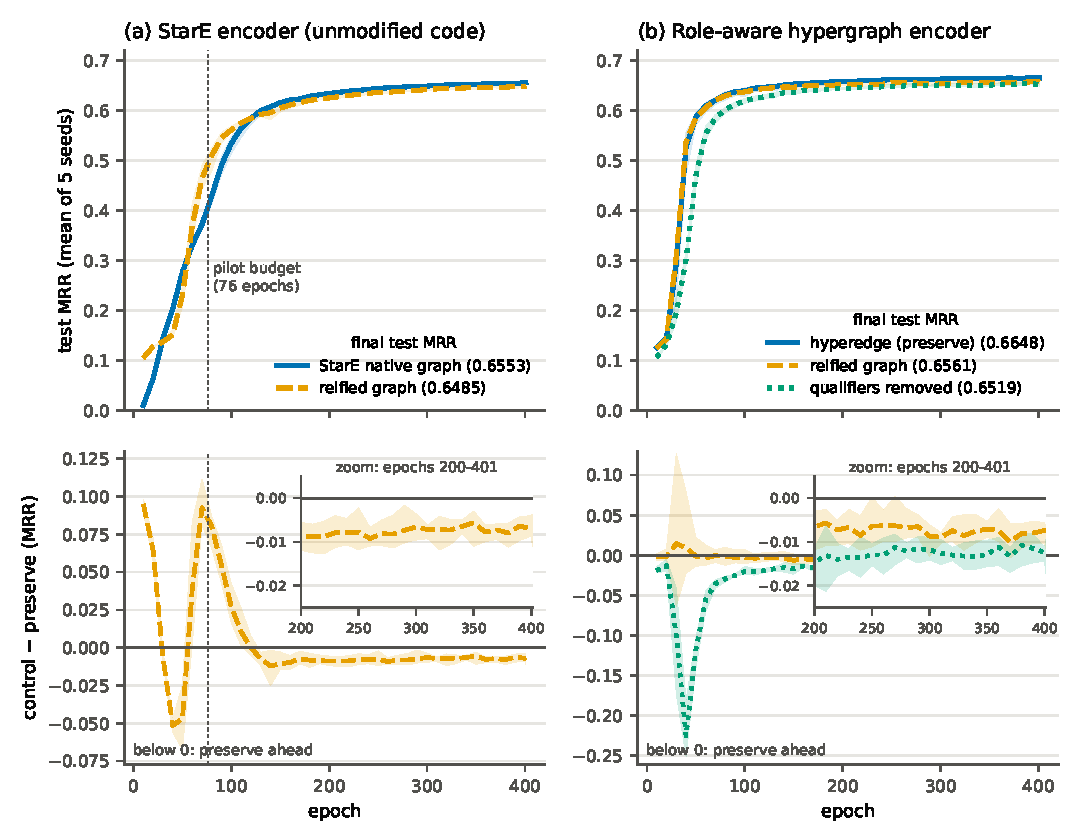
\includegraphics[width=\linewidth]{paper1_fig4_standard_protocol_curves.pdf}
\caption{Test MRR during training under the standard protocol (mean of five seeds; bands span the seeds). Top: MRR. Bottom: paired difference from the preserved or native graph; the insets zoom into epochs 200--401. (a) Study 2: the reified graph leads at most evaluation points before epoch 120, apart from a brief native lead at 30--50 epochs; the dotted line marks the budget of the pilot, which used the training graph and the validation set and recorded the opposite of the converged order. (b) Study 3: the reified arm tracks \hyper\ closely early and falls behind after about 100 epochs; removing qualifiers from the encoder slows learning sharply and leaves a lasting gap.}
\label{fig:curves}
\end{figure}

\subsection{Study 3: our encoder under the standard protocol}

Both comparisons favoured \hyper\ on all five seeds and on every reported metric (Table~\ref{tab:std}, lower block). Against \reif\ the MRR gap is $-0.0087$ ($p = 0.0004$); against \prune\ it is $-0.0129$ ($p = 0.0010$). Hits@1, Hits@3 and mean rank point the same way on 5/5 seeds for both controls. The reified arm keeps pace with \hyper\ for the first 70 epochs, leading only at epochs 30--40 on the seed mean, and falls behind after about 100 (Figure~\ref{fig:curves}b); at the final epoch \hyper\ is the best of the three arms on every seed. Removing qualifiers from the encoder slows learning markedly (mean MRR 0.469 vs.\ 0.587 at epoch 50) and the gap persists after convergence, even though the decoder of all three arms receives the qualifier tokens.

\subsection{Position among published models}
\label{sec:position}

Table~\ref{tab:position} places Studies~2 and~3 among published results on WD50K(100) under the same protocol. Our encoder sits at the level of StarE; its 0.0095 margin over StarE is not a judged comparison and comes with 4.9\% more parameters, so we do not claim it. HAHE and MAYPL did not report WD50K(100); the GLoRE authors re-ran both, and their Figure~5 places HAHE at about 0.670 and MAYPL at about 0.658---on either side of our encoder---and GLoRE at about 0.824, far above all of them \citep{ji2026glore}. A gap of about 0.005 is too small to order models whose protocols may differ, which is why we ran HAHE on our pipeline. Study~1's WD50K number (0.147) does not belong in this table: it masks any role including qualifier values, ranks all 18,025 entities of its loader, trains for 1,500 steps of 32 facts at $d=64$ rather than about 17.5 million row updates at $d=200$, and scores a 2,000-fact sample.

\begin{table}[t]
\centering
\small
\begin{threeparttable}
\caption{WD50K(100), subject/object prediction, filtered, test set.}
\label{tab:position}
\begin{tabular}{@{}lccl@{}}
\toprule
Model & MRR & Hits@10 & Source \\
\midrule
Transformer (T), no qualifiers & 0.351 & 0.530 & \citet{galkin2020stare} \\
StarE (T), no qualifiers & 0.380 & 0.584 & \citet{galkin2020stare} \\
NaLP-Fix & 0.458 & 0.563 & \citet{galkin2020stare} \\
HINGE & 0.492 & 0.636 & \citet{galkin2020stare} \\
Transformer (H) & 0.562 & 0.677 & \citet{galkin2020stare} \\
StarE (H) & 0.654 & 0.777 & \citet{galkin2020stare} \\
\midrule
StarE native graph, our run (5 seeds) & 0.6553 & 0.7766 & Study 2 \\
StarE reified graph (5 seeds) & 0.6485 & 0.7708 & Study 2 \\
Our encoder, \prune\ (5 seeds) & 0.6519 & 0.7709 & Study 3 \\
Our encoder, \reif\ (5 seeds) & 0.6561 & 0.7686 & Study 3 \\
Our encoder, \hyper\ (5 seeds) & 0.6648 & 0.7777 & Study 3 \\
HAHE, our run on the same pipeline (5 seeds)\tnote{b} & 0.6784 & 0.7947 & This paper \\
\midrule
MAYPL, re-run by \citet{ji2026glore}\tnote{a} & $\approx$0.658 & --- & \citet{ji2026glore}, Fig.~5(a) \\
HAHE, re-run by \citet{ji2026glore}\tnote{a} & $\approx$0.670 & --- & \citet{ji2026glore}, Fig.~5(a) \\
GLoRE\tnote{a} & $\approx$0.824 & --- & \citet{ji2026glore}, Fig.~5(a) \\
\bottomrule
\end{tabular}
\begin{tablenotes}\footnotesize
\item[a] The GLoRE paper reports WD50K(100) only as a figure. We read the marker positions of Figure~5(a) (main entities) from the page rendered at 400 dpi against its grid lines; the read values reproduce the figure's printed margin of GLoRE over HAHE (+0.153, +23\%) to within 0.001, and we estimate the reading error at about $\pm$0.003.
\item[b] HAHE's public code at a pinned commit, unmodified, with its published WD50K hyperparameters (not tuned) for 300 epochs, on the same rows, queries, candidates and scoring as Studies~2 and~3 (Section~\ref{sec:hahe-design}); judged against \hyper\ in Table~\ref{tab:hahe}. Under HAHE's own ranking (all 18,791 entities as candidates, ties counted against the target) the mean MRR is 0.6778.
\end{tablenotes}
\end{threeparttable}
\end{table}

\paragraph{HAHE on the same pipeline.}
HAHE beat our encoder on both judged metrics on all five seeds (Table~\ref{tab:hahe}): MRR $+0.0135$ (95\% CI $+0.0103$ to $+0.0168$) and Hits@10 $+0.0170$ ($+0.0130$ to $+0.0210$). The port reproduces the literature: under HAHE's own ranking rule its mean MRR is 0.6778, $+0.008$ from the GLoRE re-run. Two details qualify the lead. It comes from subject prediction ($+0.0305$ MRR, 5/5 seeds); on object prediction our encoder is ahead on four of five seeds ($-0.0034$). And HAHE's mean rank is worse on every seed (411.9 vs.\ 357.3): it ranks more answers near the top but pushes the answers it misses further down. The unmatched budgets do not explain the result, since HAHE's test MRR passes our encoder's final value by epoch 20 and changes little after epoch 50. HAHE differs from our encoder in size, in its fact-level Transformer and in its training objective, and we did not separate these. HAHE also keeps each fact whole, so its lead bears on the encoder, not on preservation versus reification; whether HAHE loses accuracy on the reified graph is untested. Under an identical pipeline our encoder sits below HAHE. It is a vehicle for a controlled comparison, not a competitor.

\begin{table}[t]
\centering
\small
\begin{threeparttable}
\caption{Our encoder (\hyper, epoch 401) and HAHE (epoch 300) on the identical pipeline: WD50K(100), StarE's ranking rule, test set, mean over seeds 1--5. Difference = HAHE $-$ \hyper. MRR and Hits@10 are judged; the other rows are reported. Object and subject MRR split the test queries by which position is masked. Per-seed values are in Appendix~\ref{app:seeds}.}
\label{tab:hahe}
\begin{tabular}{@{}lcccc@{}}
\toprule
 & \hyper & HAHE & Difference [95\% CI] & HAHE ahead \\
\midrule
MRR & 0.6648 $\pm$ 0.0026 & \textbf{0.6784 $\pm$ 0.0017} & $+0.0135$ [$+0.0103$, $+0.0168$] & 5/5 \\
Hits@10 & 0.7777 $\pm$ 0.0017 & \textbf{0.7947 $\pm$ 0.0028} & $+0.0170$ [$+0.0130$, $+0.0210$] & 5/5 \\
Hits@1 & 0.6025 & \textbf{0.6152} & $+0.0127$ & 5/5 \\
Mean rank\tnote{a} & \textbf{357.3} & 411.9 & $+54.6$ & 0/5 \\
\midrule
Object MRR & \textbf{0.6757} & 0.6723 & $-0.0034$ & 1/5 \\
Subject MRR & 0.6539 & \textbf{0.6844} & $+0.0305$ & 5/5 \\
\midrule
Parameters & 5,318,216 & 26,584,063 & & \\
\bottomrule
\end{tabular}
\begin{tablenotes}\footnotesize
\item[a] Lower is better; HAHE's mean rank is worse on every seed.
\end{tablenotes}
\end{threeparttable}
\end{table}

\subsection{Cost}

Reification enlarges the graph. On WD50K(100) the reified graph used 1.7$\times$ the GPU memory in Study~1 (970 vs.\ 569 MB), 1.5$\times$ in Study~2 (1,537 vs.\ 1,022 MB) and 2.2$\times$ in Study~3 (2,850 vs.\ 1,309 MB), and in Study~3 it took 30\% longer per epoch (42.8 vs.\ 33.0~s). In Study~2 the reified arm was faster (36.1 vs.\ 47.2~s per epoch) because StarE's native encoder spends time on qualifier aggregation that the reified arm does not need. HAHE is heavier than our encoder: five times the parameters, 4,023 vs.\ 1,309~MB of GPU memory, and 114.3 vs.\ 33.0~s of training compute per epoch, about 2.6 times the compute per run despite its shorter budget.

\FloatBarrier
\section{Discussion}

\paragraph{What the evidence supports.}
The same direction appeared in all nine judged comparisons and in the report-only condition, with two encoders, two protocols and two budgets, on 5/5 seeds each time. Under the standard protocol and budget the gaps are small (0.007--0.013 MRR) and their size is not the evidence; their consistency is. We read the result as: \emph{for the two message-passing encoders we tested, the standard reification of an n-ary fact is a slightly worse input than the fact itself; in Study~1's synthetic setting the difference did not come from the output head or from effective depth, and across studies it did not come from the text encoder or from a short budget}.

\paragraph{Why preservation helps.}
In the reified graph, members of a fact meet only through the statement node, two hops apart, and the fact's state is an ordinary node that is updated only after a further layer. The depth condition shows that the number of hops alone is not the reason: four layers did not close the gap in Study~1. In Study~3 both \hyper\ and \reif\ let qualifier values receive messages, so ``qualifier values are updated'' is not the reason either. The difference that remains is where the fact's state lives: as an edge state updated jointly with its members (\hyper), or as an ordinary node competing with entity nodes for the same message-passing capacity (\reif). We offer this as a hypothesis; none of our studies isolates it.

\paragraph{Budget and the direction of comparisons.}
With StarE's encoder, short budgets favoured the reified graph: it led at most evaluation points before epoch 120, by about 0.09 MRR at 70--80 epochs. With our encoder the reified arm led only at epochs 30--40, and in Study~1 \hyper\ led by a wide margin at a short budget. The early advantage is therefore a property of the StarE pairing, not of reification in general. It still matters for anyone comparing representations: a comparison stopped early can report the opposite of the converged order.

\paragraph{Does qualifier structure matter at all?}
\citet{wang2025understanding} report that a qualifier-free NBFNet matches or exceeds hyper-relational models on WD50K. In Study~3 removing qualifiers from the encoder lost on all five seeds even though the decoder still saw them. The two results are not in conflict: WD50K(100) has qualifiers on every statement while WD50K has them on 13.6\%, and the models differ. We conclude only that, on a dataset where qualifiers are dense, encoder-side qualifier structure is not replaced by decoder-side qualifier tokens.

\paragraph{What we do not claim.}
\emph{Retrieval.} In Study~1, the structure-free \textsf{flat\_text} line beat \hyper\ at retrieval under the frozen sentence encoder (recall@5 0.897 vs.\ 0.846), as the charter had predicted, while losing badly at completion (0.236 vs.\ 0.405). Finding a fact and binding its participants are different abilities (Figure~\ref{fig:strengths}); recall@5 served only to compare the two structured representations. \emph{Accuracy.} The encoder is not a state-of-the-art model: on the identical pipeline it is below HAHE on all five seeds, and it is far below GLoRE (Table~\ref{tab:position}); only the HAHE comparison is judged, and the rest of the position is descriptive. \emph{Generality.} Two encoders and two datasets (one synthetic, one Wikidata) do not support ``on any backbone'' or ``on any knowledge graph''. \emph{Language models.} We also pre-registered an attempt to inject the encoder's states into a frozen decoder-only language model \citep{qwen2024} as an alternative to retrieval-augmented generation \citep{lewis2020rag}. All six cycles failed: the best arm reached 0.244 on multi-constraint questions, below a plain list of the retrieved entity names (0.400). The advantage measured here is an encoder-level property and stops there.

\begin{figure}[t]
\centering
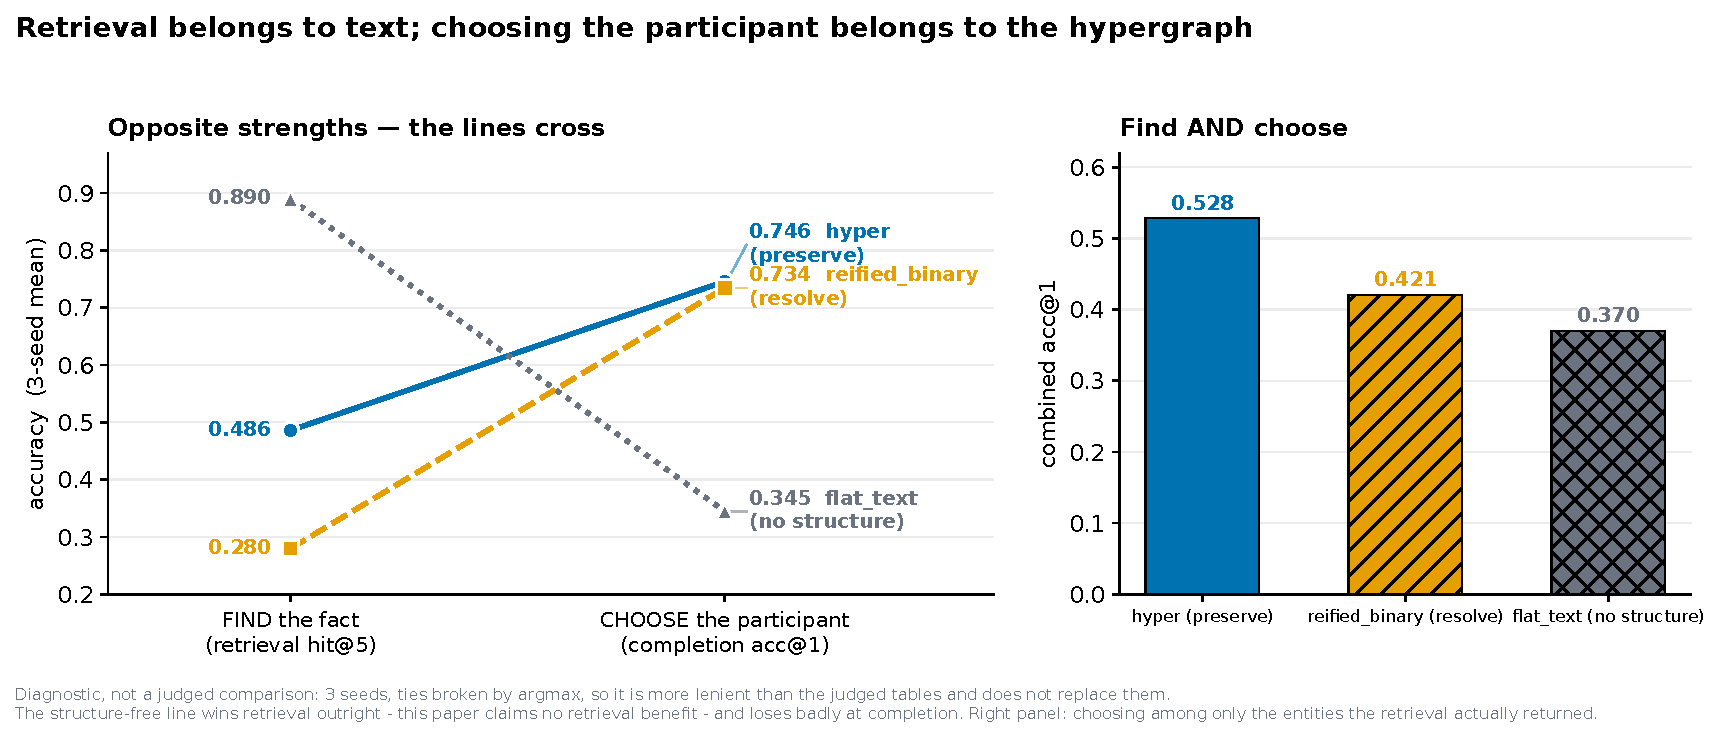
\includegraphics[width=0.92\linewidth]{paper1_fig3_opposite_strengths.pdf}
\caption{Finding a fact and choosing its participants are different abilities (Study~1 diagnostic, three seeds, ties broken by argmax; not a judged result). The structure-free text encoder ranks first at retrieval and last at completion; \hyper\ ranks first at completion and second at retrieval.}
\label{fig:strengths}
\end{figure}

\paragraph{Limitations.}
(i) Real data is a single dataset, WD50K(100), where every statement has qualifiers---the setting most favourable to qualifier structure. (ii) Studies~2 and~3 hold the budget and the hyperparameters at StarE's defaults, which StarE's authors tuned for its native graph; no arm was tuned, and how the converged gap scales with model size is untested. (iii) Study~2's gap (0.007 MRR) could in part reflect the native arm's 80,000 extra qualifier-aggregation weights (1.6\% of its parameters), which we did not control; Study~3's arms have 4.9\% more parameters than StarE, so the cross-study position in Table~\ref{tab:position} is descriptive. (iv) Our encoder keeps one representation per entity, the node-level design that GLoRE's authors report confuses roles; a pair-level encoder might show a different gap. (v) Tests are at the seed level with $n = 5$; per-query predictions were not stored, so query-level tests were not run. (vi) Plans are documented in the repository rather than on a third-party registry, and for several of them the evidence that they preceded the results is the repository's own event log (Section~\ref{sec:judging}). (vii) We ran HAHE only with its published WD50K hyperparameters, set for the full WD50K rather than WD50K(100), and for 300 epochs against our encoder's 401 (its test MRR passes our encoder's final value by epoch 20 and is flat after epoch 50). We did not run MAYPL, KREPE or GLoRE; their WD50K(100) results exist only as a figure in the GLoRE paper, from which we read them, and the MAYPL value is that paper's re-run.

\section{Conclusion}

Holding the encoder, its budget and its information fixed, and its parameters fixed or within 1.6\% (except the deliberately larger control of the depth condition), keeping an n-ary fact whole---as a hyperedge, or as StarE's qualifier-carrying edge---was a better input than its standard reification in all nine judged comparisons, on two encoders and under two protocols. Under the standard protocol the advantage is about one point of MRR and is in place by epoch 120 of 401 in both studies; with StarE's encoder, reification learns faster early and can look better at short budgets. The practical advice is modest: if a model can take n-ary facts directly, giving it the reified form costs a little accuracy and more memory, and representation comparisons should be judged at convergence. The evidence concerns the input representation, not our encoder as a model: on an identical pipeline HAHE beats it on all five seeds.

\section*{Data and code availability}
Code (including the bridge that runs HAHE's pinned public code on the StarE pipeline), run configurations, per-epoch metrics, judgment files and the plan of each study (in Korean) are available at \url{https://github.com/booobing/preserve-do-not-reify}. WD50K(100) is part of the StarE release \citep{galkin2020stare}. Every number in this manuscript is checked against the run artifacts by a script in the repository.

\section*{Declaration of generative AI use}
[The authors must complete this statement truthfully.] During the preparation of this work the author(s) used Claude (Anthropic) to write and debug experiment code, run analyses, and draft and edit the text. After using this tool, the author(s) reviewed and edited the content and take full responsibility for the publication.

\bibliographystyle{plainnat}
\bibliography{references}

\appendix
\section{Per-seed results of Studies 2 and 3 and of the HAHE comparison}
\label{app:seeds}

\begin{table}[h]
\centering
\small
\caption{Test MRR / Hits@10 at epoch 401 for each seed.}
\begin{tabular}{@{}cccccc@{}}
\toprule
& \multicolumn{2}{c}{Study 2 (StarE)} & \multicolumn{3}{c}{Study 3 (our encoder)} \\
\cmidrule(lr){2-3}\cmidrule(lr){4-6}
Seed & native & \reif & \hyper & \reif & \prune \\
\midrule
1 & 0.6551 / 0.7751 & 0.6468 / 0.7702 & 0.6657 / 0.7803 & 0.6578 / 0.7725 & 0.6519 / 0.7698 \\
2 & 0.6566 / 0.7753 & 0.6501 / 0.7705 & 0.6651 / 0.7768 & 0.6559 / 0.7664 & 0.6556 / 0.7731 \\
3 & 0.6541 / 0.7786 & 0.6504 / 0.7714 & 0.6657 / 0.7785 & 0.6588 / 0.7699 & 0.6485 / 0.7687 \\
4 & 0.6568 / 0.7760 & 0.6458 / 0.7691 & 0.6604 / 0.7767 & 0.6525 / 0.7662 & 0.6510 / 0.7712 \\
5 & 0.6541 / 0.7777 & 0.6496 / 0.7727 & 0.6672 / 0.7764 & 0.6556 / 0.7679 & 0.6527 / 0.7715 \\
\bottomrule
\end{tabular}
\end{table}

\begin{table}[h]
\centering
\small
\caption{HAHE comparison per seed: \hyper\ at epoch 401 and HAHE at epoch 300. Columns 2--3 give MRR / Hits@10 under StarE's rule; column 4 is HAHE's MRR under its own rule; columns 5--6 give MRR by prediction direction (\hyper\ / HAHE).}
\begin{tabular}{@{}cccccc@{}}
\toprule
Seed & \hyper & HAHE & HAHE, own rule & Object & Subject \\
\midrule
1 & 0.6657 / 0.7803 & 0.6775 / 0.7974 & 0.6769 & 0.6726 / 0.6706 & 0.6589 / 0.6844 \\
2 & 0.6651 / 0.7768 & 0.6770 / 0.7945 & 0.6765 & 0.6760 / 0.6719 & 0.6542 / 0.6822 \\
3 & 0.6657 / 0.7785 & 0.6777 / 0.7902 & 0.6771 & 0.6789 / 0.6708 & 0.6525 / 0.6845 \\
4 & 0.6604 / 0.7767 & 0.6783 / 0.7948 & 0.6776 & 0.6721 / 0.6728 & 0.6487 / 0.6837 \\
5 & 0.6672 / 0.7764 & 0.6813 / 0.7967 & 0.6807 & 0.6790 / 0.6756 & 0.6553 / 0.6871 \\
\bottomrule
\end{tabular}
\end{table}

\end{document}
